\begin{figure}[t]
  \centering
  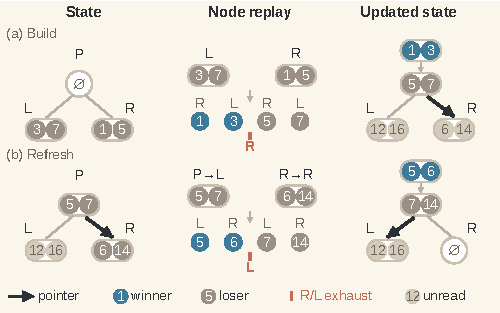
\includegraphics[width=\linewidth]{../round2/mechanisms/pointer.pdf}
  \caption{Pointer assignment for $h=2$. Scan ranked replay slots until one contributes its second item (double outline). Tree construction exhausts slot R at 5. During path refresh, retained parent P occupies slot L and the incoming right segment occupies slot R; L exhausts at 7. Slot labels are replay positions, not original run identities. Gray winners are forwarded upward; remaining items are stored at P.}
  \label{fig:pointer-mechanism}
\end{figure}
